\documentclass[a4paper]{scrartcl}
\usepackage[utf8]{inputenc}
\usepackage{amsmath,amssymb,amsthm}
\usepackage{enumitem,setspace}
\usepackage[usenames,dvipsnames,table]{xcolor}
\usepackage{graphicx}
\DeclareGraphicsExtensions{.pdf,.png,.eps,.jpg}
\usepackage{algorithm2e}
\usepackage{tikz}
\usetikzlibrary{graphs,positioning}

% --- math operators ---
\usepackage{mathtools}
\DeclarePairedDelimiter\set{\{}{\}} % use $\set{1, 2, 3}$
\DeclarePairedDelimiter\abs{\lvert}{\rvert}
\DeclarePairedDelimiter\norm{\lVert}{\rVert}
\DeclarePairedDelimiter\ceils{\lceil}{\rceil}
\DeclarePairedDelimiter\floor{\lfloor}{\rfloor}
\def\then{\ensuremath{\Rightarrow}} % =>
\def\iff{\ensuremath{\Leftrightarrow}} % if and only if <=>
\def\to{\ensuremath{\rightarrow}} % ->
\def\ot{\ensuremath{\leftarrow}} % ->
\def\Oh{\ensuremath{\mathcal{O}}} % big O like $\Oh(n)$
% ---
\DeclareMathOperator{\preorder}{preorder}
\DeclareMathOperator{\postorder}{postorder}
\DeclareMathOperator{\depth}{depth}

% --- FILL OUT THESE 3 FIELDS ---
\def\sheetNumber{1}
\def\names{Matthias Janßen, Raphael Thelen, Tillmann
Faust} 
\def\sumPoints{20} 

% --- ### BEGIN DOCUMENT ### ---
\begin{document} 

\begin{doublespace} % header
\noindent \textbf{\LARGE{Übungsblatt \sheetNumber}}
\hfill  {\large Punkte: $\boxed{\qquad  /\; \sumPoints}$}\\
{\Large \textbf{Fortgeschrittene Algorithmen (Wintersemester 2022/23)}\\
Bearbeitet von: \textbf{\names}\\
\today}
\end{doublespace}


\section*{Aufgabe 1}
a)
\begin{center}
    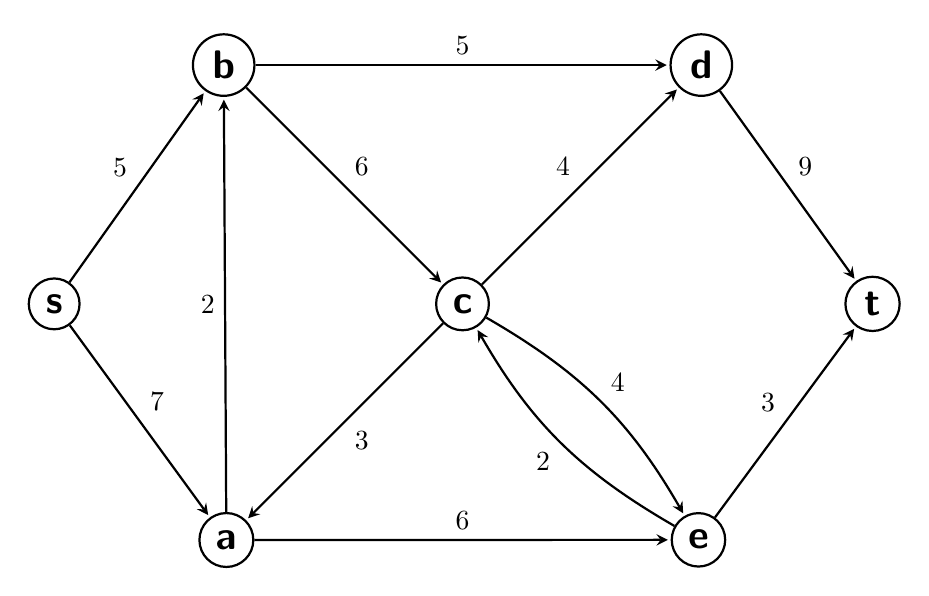
\begin{tikzpicture}[->,>=stealth,shorten >=1pt,auto,node distance=2cm,thick,
      main node/.style={circle,draw,font=\sffamily\Large\bfseries}]
      \node[main node] (c) {c};
      \node[main node] (b) [above left=2.5cm and 2.5cm of c] {b};
      \node[main node] (d) [above right=2.5cm and 2.5cm of c] {d};
      \node[main node] (e) [below right=2.5cm and 2.5cm of c] {e};
      \node[main node] (a) [below left=2.5cm and 2.5cm of c] {a};
      \node[main node] (s) [left=4.5cm of c] {s};
      \node[main node] (t) [right=4.5cm of c] {t};

      \path[->]
        (s) edge node {5} (b)
        (s) edge node {7} (a)
        (a) edge node {2} (b)
        (a) edge node {6} (e)
        (b) edge node {5} (d)
        (b) edge node {6} (c)
        (c) edge node {4} (d)
        (c) edge node {3} (a)
        (c) edge [bend left=15] node {4} (e)
        (e) edge [bend left=15] node {2} (c)
        (d) edge node {9} (t)
        (e) edge node {3} (t);
    \end{tikzpicture}
    Fluss = 0
    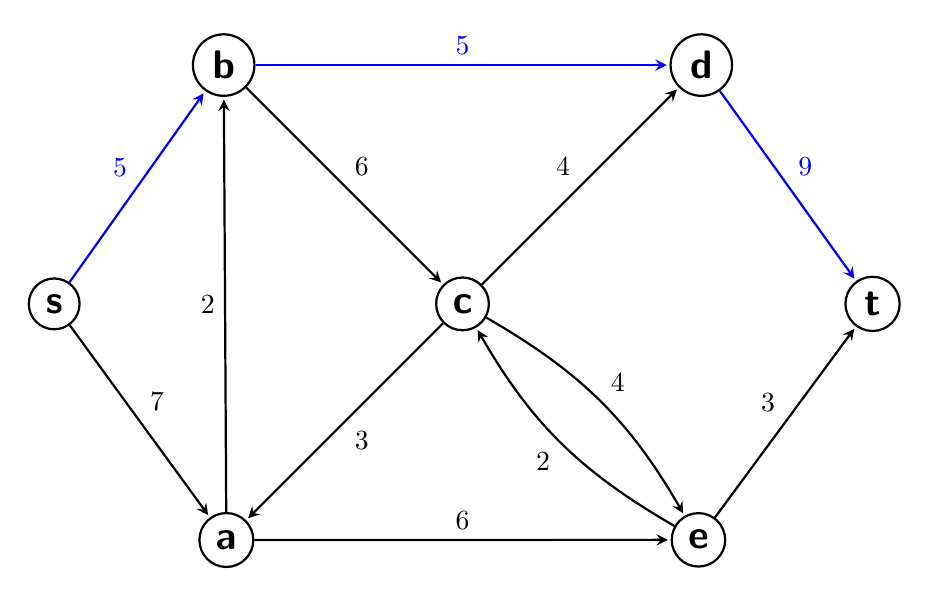
\begin{tikzpicture}[->,>=stealth,shorten >=1pt,auto,node distance=2cm,thick,
      main node/.style={circle,draw,font=\sffamily\Large\bfseries}]
      \node[main node] (c) {c};
      \node[main node] (b) [above left=2.5cm and 2.5cm of c] {b};
      \node[main node] (d) [above right=2.5cm and 2.5cm of c] {d};
      \node[main node] (e) [below right=2.5cm and 2.5cm of c] {e};
      \node[main node] (a) [below left=2.5cm and 2.5cm of c] {a};
      \node[main node] (s) [left=4.5cm of c] {s};
      \node[main node] (t) [right=4.5cm of c] {t};

      \path[->]
        (s) edge [blue] node {5} (b)
        (s) edge node {7} (a)
        (a) edge node {2} (b)
        (a) edge node {6} (e)
        (b) edge [blue] node {5} (d)
        (b) edge node {6} (c)
        (c) edge node {3} (a)
        (c) edge node {4} (d)
        (c) edge [bend left=15] node {4} (e)
        (d) edge [blue] node {9} (t)
        (e) edge [bend left=15] node {2} (c)
        (e) edge node {3} (t);
    \end{tikzpicture}
    Fluss = 0
    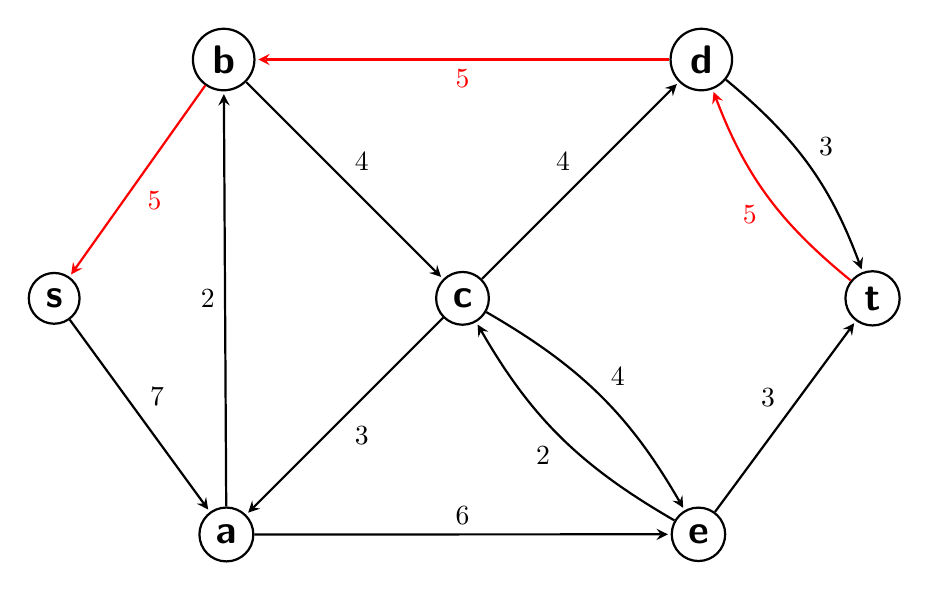
\begin{tikzpicture}[->,>=stealth,shorten >=1pt,auto,node distance=2cm,thick,
      main node/.style={circle,draw,font=\sffamily\Large\bfseries}]
      \node[main node] (c) {c};
      \node[main node] (b) [above left=2.5cm and 2.5cm of c] {b};
      \node[main node] (d) [above right=2.5cm and 2.5cm of c] {d};
      \node[main node] (e) [below right=2.5cm and 2.5cm of c] {e};
      \node[main node] (a) [below left=2.5cm and 2.5cm of c] {a};
      \node[main node] (s) [left=4.5cm of c] {s};
      \node[main node] (t) [right=4.5cm of c] {t};

      \path[->]
        (s) edge node {7} (a)
        (a) edge node {2} (b)
        (a) edge node {6} (e)
        (b) edge node {4} (c)
        (c) edge node {3} (a)
        (c) edge [bend left=15] node {4} (e)
        (c) edge node {4} (d)
        (d) edge [bend left=15] node {3} (t)
        (e) edge [bend left=15] node {2} (c)
        (e) edge node {3} (t)

        (b) edge [red] node {5} (s)
        (d) edge [red] node {5} (b)
        (t) edge [bend left=15][red] node {5} (d);
    \end{tikzpicture}
    Fluss 5
    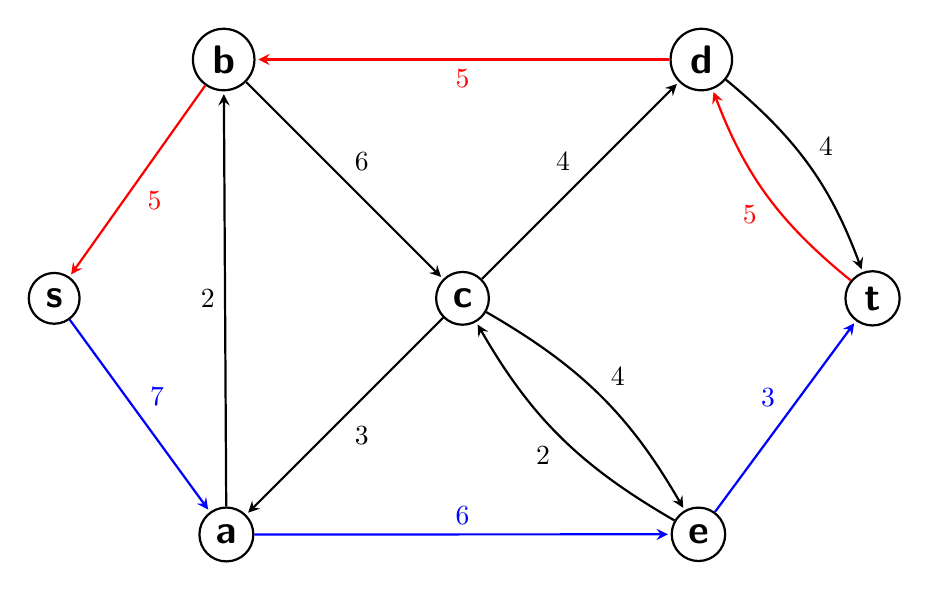
\begin{tikzpicture}[->,>=stealth,shorten >=1pt,auto,node distance=2cm,thick,
      main node/.style={circle,draw,font=\sffamily\Large\bfseries}]
      \node[main node] (c) {c};
      \node[main node] (b) [above left=2.5cm and 2.5cm of c] {b};
      \node[main node] (d) [above right=2.5cm and 2.5cm of c] {d};
      \node[main node] (e) [below right=2.5cm and 2.5cm of c] {e};
      \node[main node] (a) [below left=2.5cm and 2.5cm of c] {a};
      \node[main node] (s) [left=4.5cm of c] {s};
      \node[main node] (t) [right=4.5cm of c] {t};

      \path[->]
        (s) edge [blue] node {7} (a)
        (a) edge node {2} (b)
        (a) edge [blue] node {6} (e)
        (b) edge node {6} (c)
        (c) edge node {4} (d)
        (c) edge node {3} (a)
        (c) edge [bend left=15] node {4} (e)
        (e) edge [bend left=15] node {2} (c)
        (d) edge [bend left=15] node {4} (t)
        (e) edge [blue] node {3} (t)
        
        (b) edge [red] node {5} (s)
        (d) edge [red] node {5} (b)
        (t) edge [bend left=15][red] node {5} (d);
    \end{tikzpicture} 
    Fluss = 5
    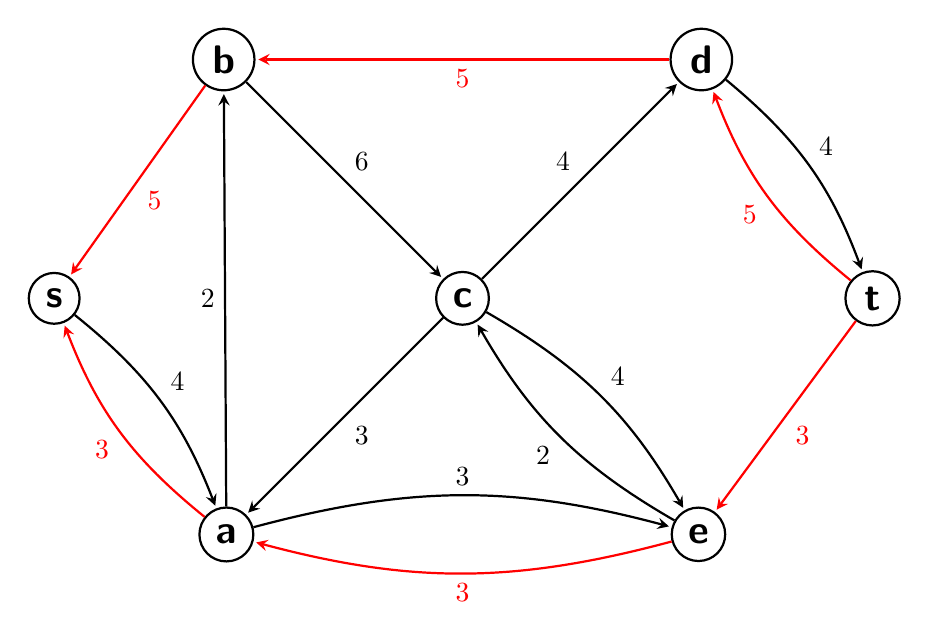
\begin{tikzpicture}[->,>=stealth,shorten >=1pt,auto,node distance=2cm,thick,
      main node/.style={circle,draw,font=\sffamily\Large\bfseries}]
      \node[main node] (c) {c};
      \node[main node] (b) [above left=2.5cm and 2.5cm of c] {b};
      \node[main node] (d) [above right=2.5cm and 2.5cm of c] {d};
      \node[main node] (e) [below right=2.5cm and 2.5cm of c] {e};
      \node[main node] (a) [below left=2.5cm and 2.5cm of c] {a};
      \node[main node] (s) [left=4.5cm of c] {s};
      \node[main node] (t) [right=4.5cm of c] {t};

      \path[->]
        (s) edge [bend left=15] node {4} (a)
        (a) edge node {2} (b)
        (a) edge [bend left=15] node {3} (e)
        (b) edge node {6} (c)
        (c) edge node {4} (d)
        (c) edge node {3} (a)
        (c) edge [bend left=15] node {4} (e)
        (e) edge [bend left=15] node {2} (c)
        (d) edge [bend left=15] node {4} (t)

        (b) edge [red] node {5} (s)
        (d) edge [red] node {5} (b)
        (t) edge [bend left=15][red] node {5} (d)
        (a) edge [bend left=15][red] node {3} (s)
        (e) edge [bend left=15][red] node {3} (a)
        (t) edge [red] node {3} (e);
    \end{tikzpicture} 
    Fluss = 8
    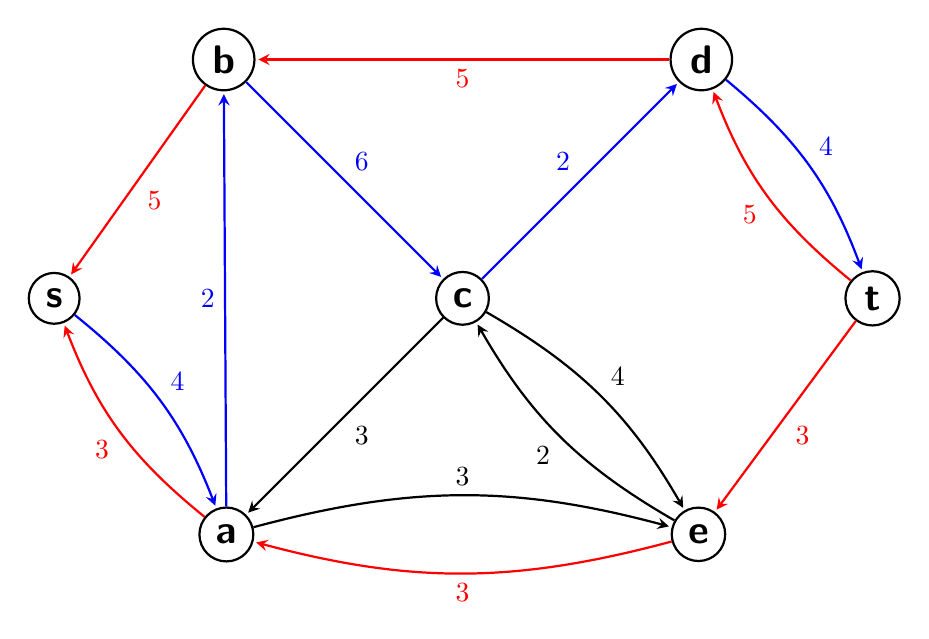
\begin{tikzpicture}[->,>=stealth,shorten >=1pt,auto,node distance=2cm,thick,
      main node/.style={circle,draw,font=\sffamily\Large\bfseries}]
      \node[main node] (c) {c};
      \node[main node] (b) [above left=2.5cm and 2.5cm of c] {b};
      \node[main node] (d) [above right=2.5cm and 2.5cm of c] {d};
      \node[main node] (e) [below right=2.5cm and 2.5cm of c] {e};
      \node[main node] (a) [below left=2.5cm and 2.5cm of c] {a};
      \node[main node] (s) [left=4.5cm of c] {s};
      \node[main node] (t) [right=4.5cm of c] {t};

      \path[->]
        (s) edge [bend left=15][blue] node {4} (a)
        (a) edge [blue] node {2} (b)
        (a) edge [bend left=15] node {3} (e)
        (b) edge [blue] node {6} (c)
        (c) edge [blue] node {2} (d)
        (c) edge node {3} (a)
        (c) edge [bend left=15] node {4} (e)
        (e) edge [bend left=15] node {2} (c)
        (d) edge [bend left=15][blue] node {4} (t)
        
        (b) edge [red] node {5} (s)
        (d) edge [red] node {5} (b)
        (t) edge [bend left=15][red] node {5} (d)
        (a) edge [bend left=15][red] node {3} (s)
        (e) edge [bend left=15][red] node {3} (a)
        (t) edge [red] node {3} (e);
    \end{tikzpicture}
    Fluss = 8
    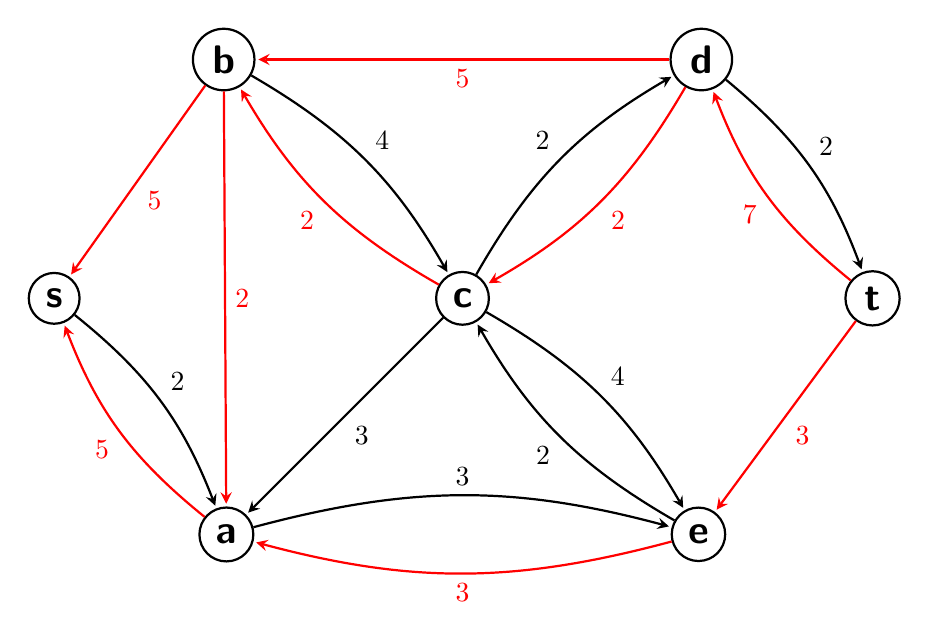
\begin{tikzpicture}[->,>=stealth,shorten >=1pt,auto,node distance=2cm,thick,
      main node/.style={circle,draw,font=\sffamily\Large\bfseries}]
      \node[main node] (c) {c};
      \node[main node] (b) [above left=2.5cm and 2.5cm of c] {b};
      \node[main node] (d) [above right=2.5cm and 2.5cm of c] {d};
      \node[main node] (e) [below right=2.5cm and 2.5cm of c] {e};
      \node[main node] (a) [below left=2.5cm and 2.5cm of c] {a};
      \node[main node] (s) [left=4.5cm of c] {s};
      \node[main node] (t) [right=4.5cm of c] {t};

      \path[->]
        (s) edge [bend left=15] node {2} (a)
        (a) edge [bend left=15] node {3} (e)
        (b) edge [bend left=15] node {4} (c)
        (c) edge [bend left=15] node {2} (d)
        (c) edge node {3} (a)
        (c) edge [bend left=15] node {4} (e)
        (e) edge [bend left=15] node {2} (c)
        (d) edge [bend left=15] node {2} (t)
        
        (b) edge [red] node {5} (s)
        (b) edge [red] node {2} (a)
        (c) edge [bend left=15][red] node {2} (b)
        (d) edge [red] node {5} (b)
        (d) edge [bend left=15][red] node {2} (c)
        (t) edge [bend left=15][red] node {7} (d)
        (a) edge [bend left=15][red] node {5} (s)
        (e) edge [bend left=15][red] node {3} (a)
        (t) edge [red] node {3} (e);
    \end{tikzpicture}
    Fluss = 12
    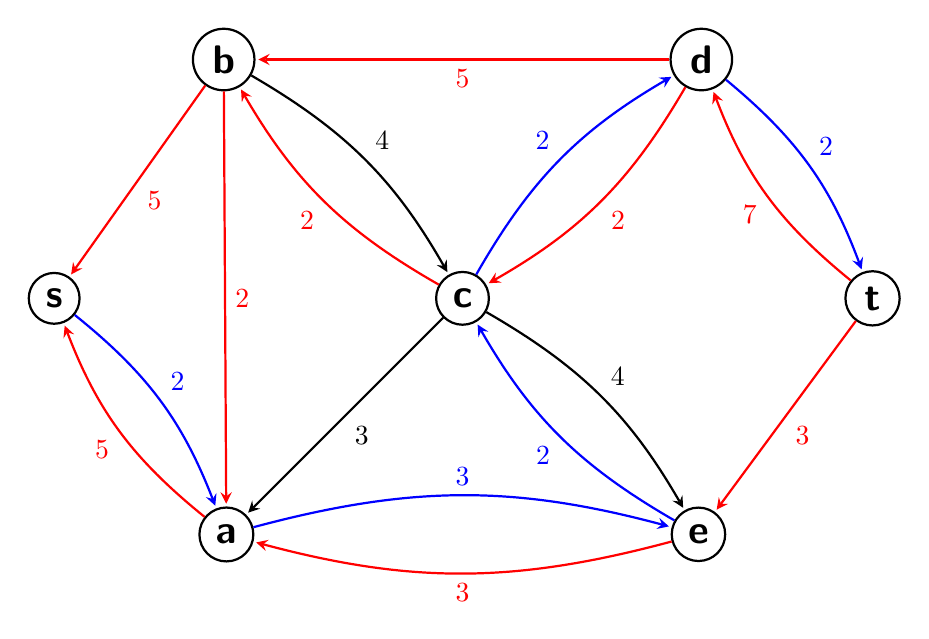
\begin{tikzpicture}[->,>=stealth,shorten >=1pt,auto,node distance=2cm,thick,
      main node/.style={circle,draw,font=\sffamily\Large\bfseries}]
      \node[main node] (c) {c};
      \node[main node] (b) [above left=2.5cm and 2.5cm of c] {b};
      \node[main node] (d) [above right=2.5cm and 2.5cm of c] {d};
      \node[main node] (e) [below right=2.5cm and 2.5cm of c] {e};
      \node[main node] (a) [below left=2.5cm and 2.5cm of c] {a};
      \node[main node] (s) [left=4.5cm of c] {s};
      \node[main node] (t) [right=4.5cm of c] {t};

      \path[->]
        (s) edge [bend left=15][blue] node {2} (a)
        (a) edge [bend left=15][blue] node {3} (e)
        (b) edge [bend left=15] node {4} (c)
        (c) edge [bend left=15][blue] node {2} (d)
        (c) edge node {3} (a)
        (c) edge [bend left=15] node {4} (e)
        (e) edge [bend left=15][blue] node {2} (c)
        (d) edge [bend left=15][blue] node {2} (t)
        
        (b) edge [red] node {5} (s)
        (b) edge [red] node {2} (a)
        (c) edge [bend left=15][red] node {2} (b)
        (d) edge [red] node {5} (b)
        (d) edge [bend left=15][red] node {2} (c)
        (t) edge [bend left=15][red] node {7} (d)
        (a) edge [bend left=15][red] node {5} (s)
        (e) edge [bend left=15][red] node {3} (a)
        (t) edge [red] node {3} (e);
    \end{tikzpicture}
    Fluss = 10
    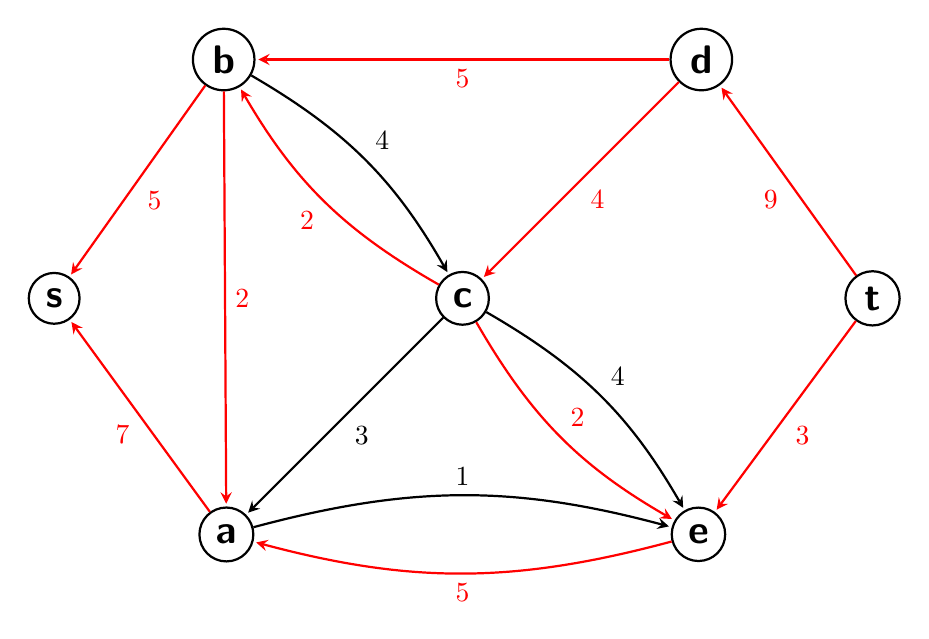
\begin{tikzpicture}[->,>=stealth,shorten >=1pt,auto,node distance=2cm,thick,
      main node/.style={circle,draw,font=\sffamily\Large\bfseries}]
      \node[main node] (c) {c};
      \node[main node] (b) [above left=2.5cm and 2.5cm of c] {b};
      \node[main node] (d) [above right=2.5cm and 2.5cm of c] {d};
      \node[main node] (e) [below right=2.5cm and 2.5cm of c] {e};
      \node[main node] (a) [below left=2.5cm and 2.5cm of c] {a};
      \node[main node] (s) [left=4.5cm of c] {s};
      \node[main node] (t) [right=4.5cm of c] {t};

      \path[->]
        (a) edge [bend left=15] node {1} (e)
        (b) edge [bend left=15] node {4} (c)
        (c) edge node {3} (a)
        (c) edge [bend left=15] node {4} (e)

        (b) edge [red] node {5} (s)
        (b) edge [red] node {2} (a)
        (c) edge [bend left=15][red] node {2} (b)
        (d) edge [red] node {5} (b)
        (d) edge [red] node {4} (c)
        (t) edge [red] node {9} (d)
        (a) edge [red] node {7} (s)
        (e) edge [bend left=15][red] node {5} (a)
        (t) edge [red] node {3} (e)
        (c) edge [bend right=15][red] node {2} (e);
    \end{tikzpicture}
    Fluss = 12
\end{center}
Es existiert kein weiterer augmentierender Pfad von s nach t.
Der maximale Fluss in dem gegebenen Graphen ist daher 12.
\\\\
b)
\begin{center}
    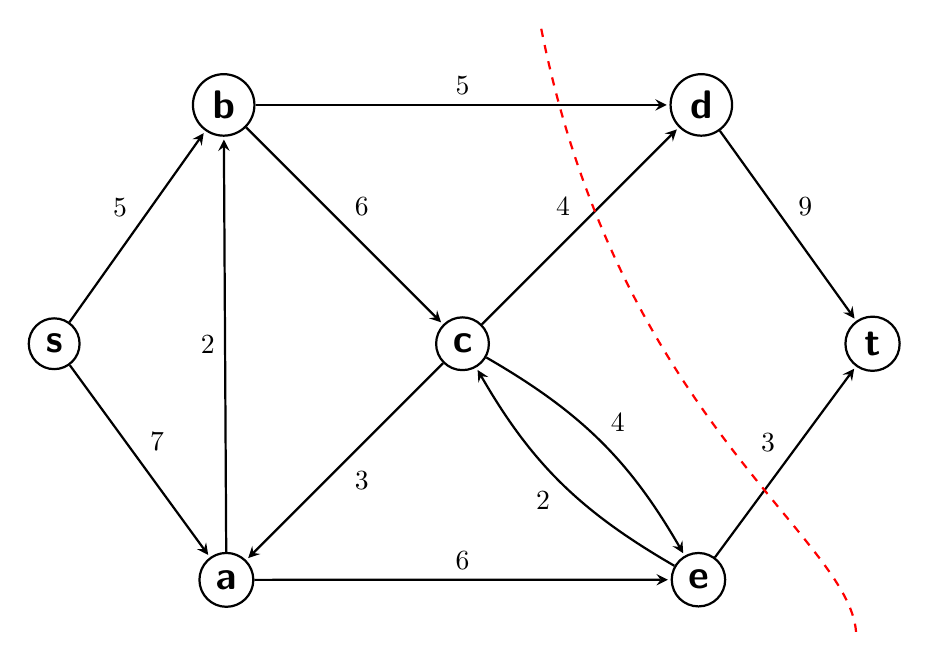
\begin{tikzpicture}[>=stealth,shorten >=1pt,auto,node distance=2cm,thick,
      main node/.style={circle,draw,font=\sffamily\Large\bfseries}]
      \node[main node] (c) {c};
      \node[main node] (b) [above left=2.5cm and 2.5cm of c] {b};
      \node[main node] (d) [above right=2.5cm and 2.5cm of c] {d};
      \node[main node] (e) [below right=2.5cm and 2.5cm of c] {e};
      \node[main node] (a) [below left=2.5cm and 2.5cm of c] {a};
      \node[main node] (s) [left=4.5cm of c] {s};
      \node[main node] (t) [right=4.5cm of c] {t};

      \path[->]
        (s) edge node {5} (b)
        (s) edge node {7} (a)
        (a) edge node {2} (b)
        (a) edge node {6} (e)
        (b) edge node {5} (d)
        (b) edge node {6} (c)
        (c) edge node {4} (d)
        (c) edge node {3} (a)
        (c) edge [bend left=15] node {4} (e)
        (e) edge [bend left=15] node {2} (c)
        (d) edge node {9} (t)
        (e) edge node {3} (t);

        \draw[dashed][red] (1,4) .. controls (2,-1) and (5,-2.5) .. (5,-3.75);
    \end{tikzpicture}
\end{center}
Der eingezeichnete Schnitt ist minimal und hat die Kapazität 12, was dem maximalen Fluss entspricht.
\\\\
c)
Alle Knoten im Graphen sind von s aus erreichbar. Es gibt keine Kante, die von einem erreichbaren Knoten zu einem nicht erreichbaren Knoten führt.
Ein S,T SChnitt ist daher immer zusammenhängend.
\section*{Aufgabe 2}

\section*{Aufgabe 3}

\section*{Aufgabe 4}


% -- code for figures
% \begin{figure}[htb]
% \centering
% \includegraphics{filename} % use option [width=\linewidth] to change size to linewidth (or 0.6\linewidth for example)
% \label{fig:name}
% \end{figure}


\end{document}
% --- ### END DOCUMENT ### ---